%%%%%%%%%%%%%%%%%%%%%%%%%%%%%%%%%%%%%%%%%
% Structured General Purpose Assignment
% LaTeX Template
%
% This template has been downloaded from:
% http://www.latextemplates.com
%
% Original author:
% Ted Pavlic (http://www.tedpavlic.com)
%
% Note:
% The \lipsum[#] commands throughout this template generate dummy text
% to fill the template out. These commands should all be removed when 
% writing assignment content.
%
%%%%%%%%%%%%%%%%%%%%%%%%%%%%%%%%%%%%%%%%%

%----------------------------------------------------------------------------------------
%	PACKAGES AND OTHER DOCUMENT CONFIGURATIONS
%----------------------------------------------------------------------------------------

\documentclass{article}

\usepackage{fancyhdr} % Required for custom headers
\usepackage{lastpage} % Required to determine the last page for the footer
\usepackage{extramarks} % Required for headers and footers
\usepackage{graphicx} % Required to insert images
\usepackage{lipsum} % Used for inserting dummy 'Lorem ipsum' text into the template
\usepackage{amsmath}
\usepackage{subcaption}
\usepackage{caption}
\usepackage{float}


% Margins
\topmargin=-0.45in
\evensidemargin=0in
\oddsidemargin=0in
\textwidth=6.5in
\textheight=9.0in
\headsep=0.25in 

\linespread{1.1} % Line spacing

% Set up the header and footer
\pagestyle{fancy}
\lhead{\hmwkAuthorName} % Top left header
\chead{\hmwkClass\ (\hmwkClassInstructor\ \hmwkClassTime): \hmwkTitle} % Top center header
\rhead{\firstxmark} % Top right header
\lfoot{\lastxmark} % Bottom left footer
\cfoot{} % Bottom center footer
\rfoot{Page\ \thepage\ of\ \pageref{LastPage}} % Bottom right footer
\renewcommand\headrulewidth{0.4pt} % Size of the header rule
\renewcommand\footrulewidth{0.4pt} % Size of the footer rule
\newcommand{\twopartdef}[4]
{
	\left\{
		\begin{array}{ll}
			#1 & \mbox{if } #2 \\
			#3 & \mbox{ } #4
		\end{array}
	\right.
}

\setlength\parindent{0pt} % Removes all indentation from paragraphs

%----------------------------------------------------------------------------------------
%	DOCUMENT STRUCTURE COMMANDS
%	Skip this unless you know what you're doing
%----------------------------------------------------------------------------------------

% Header and footer for when a page split occurs within a problem environment
\newcommand\numberthis{\addtocounter{equation}{1}\tag{\theequation}}
\newcommand{\enterProblemHeader}[1]{
\nobreak\extramarks{#1}{#1 continued on next page\ldots}\nobreak
\nobreak\extramarks{#1 (continued)}{#1 continued on next page\ldots}\nobreak
}

% Header and footer for when a page split occurs between problem environments
\newcommand{\exitProblemHeader}[1]{
\nobreak\extramarks{#1 (continued)}{#1 continued on next page\ldots}\nobreak
\nobreak\extramarks{#1}{}\nobreak
}

\setcounter{secnumdepth}{0} % Removes default section numbers
\newcounter{homeworkProblemCounter} % Creates a counter to keep track of the number of problems

\newcommand{\homeworkProblemName}{}
\newenvironment{homeworkProblem}[1][Problem \arabic{homeworkProblemCounter}]{ % Makes a new environment called homeworkProblem which takes 1 argument (custom name) but the default is "Problem #"
\stepcounter{homeworkProblemCounter} % Increase counter for number of problems
\renewcommand{\homeworkProblemName}{#1} % Assign \homeworkProblemName the name of the problem
\section{\homeworkProblemName} % Make a section in the document with the custom problem count
\enterProblemHeader{\homeworkProblemName} % Header and footer within the environment
}{
\exitProblemHeader{\homeworkProblemName} % Header and footer after the environment
}

\newcommand{\problemAnswer}[1]{ % Defines the problem answer command with the content as the only argument
\noindent\framebox[\columnwidth][c]{\begin{minipage}{0.98\columnwidth}#1\end{minipage}} % Makes the box around the problem answer and puts the content inside
}

\newcommand{\homeworkSectionName}{}
\newenvironment{homeworkSection}[1]{ % New environment for sections within homework problems, takes 1 argument - the name of the section
\renewcommand{\homeworkSectionName}{#1} % Assign \homeworkSectionName to the name of the section from the environment argument
\subsection{\homeworkSectionName} % Make a subsection with the custom name of the subsection
\enterProblemHeader{\homeworkProblemName\ [\homeworkSectionName]} % Header and footer within the environment
}{
\enterProblemHeader{\homeworkProblemName} % Header and footer after the environment
}
   
%----------------------------------------------------------------------------------------
%	NAME AND CLASS SECTION
%----------------------------------------------------------------------------------------

\newcommand{\hmwkTitle}{Homework\ \#1} % Assignment title
\newcommand{\hmwkDueDate}{Sat.,\ Mehr\ 25,\ 1395} % Due date
\newcommand{\hmwkClass}{Statistical Pattern Recognition} % Course/class
\newcommand{\hmwkClassTime}{} % Class/lecture time
\newcommand{\hmwkClassInstructor}{Dr. Rahmati} % Teacher/lecturer
\newcommand{\hmwkAuthorName}{Ahmad Asadi} % Your name

%----------------------------------------------------------------------------------------
%	TITLE PAGE
%----------------------------------------------------------------------------------------

\title{
\vspace{2in}
\textmd{\textbf{\hmwkClass:\ \hmwkTitle}}\\
\normalsize\vspace{0.1in}\small{Due\ on\ \hmwkDueDate}\\
\vspace{0.1in}\large{\textit{\hmwkClassInstructor\ \hmwkClassTime}}
\vspace{3in}
}

\author{\textbf{\hmwkAuthorName}}
\date{} % Insert date here if you want it to appear below your name

%----------------------------------------------------------------------------------------

\begin{document}

\maketitle

%----------------------------------------------------------------------------------------
%	TABLE OF CONTENTS
%----------------------------------------------------------------------------------------

%\setcounter{tocdepth}{1} % Uncomment this line if you don't want subsections listed in the ToC

\newpage
\tableofcontents
\newpage

%----------------------------------------------------------------------------------------
%	PROBLEM 1
%----------------------------------------------------------------------------------------

% To have just one problem per page, simply put a \clearpage after each problem

\begin{homeworkProblem}
A random variable $X$ has $E(X) = 2$ and $E(X^2) = 2$. Let $Y = -2X - 5$. Compute:
\begin{enumerate}

\item $V(X)$
\item $V(Y)$
\item $E(Y^2)$
\end{enumerate}

\vspace{10pt}
\Large{Solution:}
\vspace{10pt} % Question

\problemAnswer{ % Answer
\begin{enumerate}
\item $V(X)$ :

\begin{align*}
&V(X) = E(X^2) - E(X)^2 \implies V(X) = 2 - 4 = -2. 
\end{align*}

\item $V(Y)$ :
\begin{align*}
&V(\alpha X + \beta) = \alpha^2 V(X) \implies V(Y) = V(-2X - 5) = 4 V(X) \\
&\implies V(Y) = -8.
\end{align*}

\item $E(Y^2)$ :
\begin{align*}
&E(\alpha X + \beta) = \alpha E(X) + \beta \implies E(Y) = E(-2X - 5) = -2E(X) - 5 \\
					&\implies E(Y) = -9.\\
&V(Y) = E(Y^2) - E(Y)^2 \implies E(Y^2) = V(Y) + E(Y)^2 \\
&\implies E(Y^2) = -8 - 9 = -17. 
\end{align*}

\end{enumerate}

}


\end{homeworkProblem}

%----------------------------------------------------------------------------------------
%	PROBLEM 2
%----------------------------------------------------------------------------------------

\begin{homeworkProblem}
Generate 100 samples from normal distribution specified by $\mu = 1$, $\sigma = 0.5, 1, 2$. Plot
histogram of generated samples and compare the results.


\vspace{10pt}
\Large{Solution}
\vspace{10pt}

\problemAnswer{

In figure \ref{fig:1}, the histogram of 100 generated samples from Gaussian distribution with $\mu = 1$ and $\sigma = 0.5$ has been displayed. As its obvious in this figure, the distribution of samples around the mean values is symmetric and the most of them are generated in $[-0.5 , 2]$ which is in range of twice $\sigma$ from each side around $\mu$.
\begin{figure}[H]
	\centering
	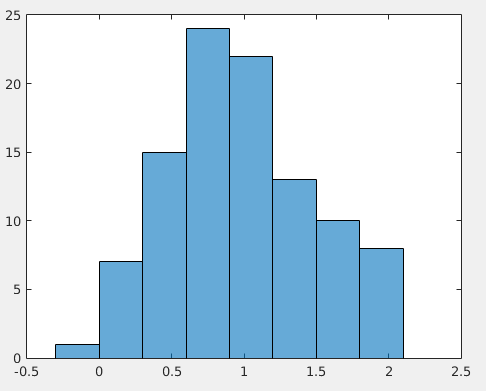
\includegraphics[scale=0.5]{Imgs/01021.png}
	\caption{Histogram for Samples from $N(1, 0.5)$}
	\label{fig:1}
\end{figure}

Also, figure \ref{fig:2}, represents the histogram of generated samples from Gaussian distribution with $\mu = 1$ and $\sigma = 1$. As it is shown in this figure, data is dense in range $[-2,4]$ which is in range of twice $\sigma$ from each side around $\mu$.
\begin{figure}[H]
	\centering
	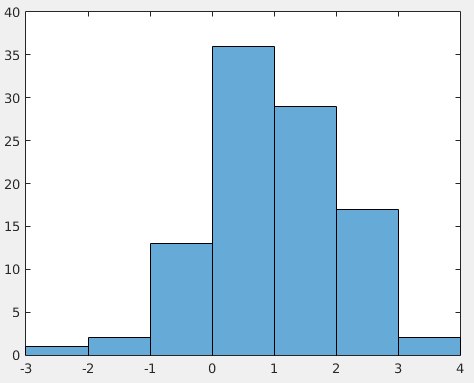
\includegraphics[scale=0.5]{Imgs/01022.png}
	\caption{Histogram for Samples from $N(1, 1)$}
	\label{fig:2}
\end{figure}
}
\problemAnswer{
Finally, figure \ref{fig:3} illustrates density of generated data from Gaussian distribution with $\mu = 1$ and $\sigma = 2$. As same as previous cases, generated samples are dense in range $[-3, 5]$, twice $\sigma$ from each side around $\mu$.

\begin{figure}[H]
	\centering
	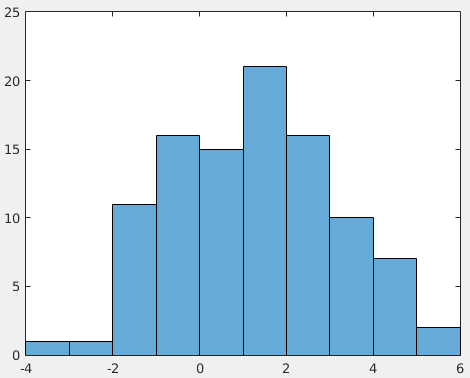
\includegraphics[scale=0.5]{Imgs/01023.png}
	\caption{Histogram for Samples from $N(1, 2)$}
	\label{fig:3}
\end{figure}

}

\end{homeworkProblem}





\begin{homeworkProblem}
Generate and plot samples from normal distribution specified by:
\begin{enumerate}
\item $\mu_1 = \left[ \begin{smallmatrix} 1 \\ 0 \end{smallmatrix} \right] $ and $\Sigma_1 = \left[ \begin{smallmatrix} 5 & 0 \\ 0 & 5  \end{smallmatrix} \right]$
\item $\mu_2 = \left[ \begin{smallmatrix} 2 \\ 0 \end{smallmatrix} \right] $ and $\Sigma_2 = \left[ \begin{smallmatrix} 5 & 0 \\ 0 & 10  \end{smallmatrix} \right]$
\item $\mu_3 = \left[ \begin{smallmatrix} -1 \\ 1 \end{smallmatrix} \right] $ and $\Sigma_3 = \left[ \begin{smallmatrix} 5 & 6 \\ 6 & 10  \end{smallmatrix} \right]$
\end{enumerate}

\vspace{10pt}
\Large{Solution}
\vspace{10pt}

\problemAnswer{

In figure \ref{fig:4}, the histogram of 100 generated samples from Gaussian distribution with $\mu_1$ and $\Sigma_1$ has been displayed. 
\begin{figure}[H]
	\centering
	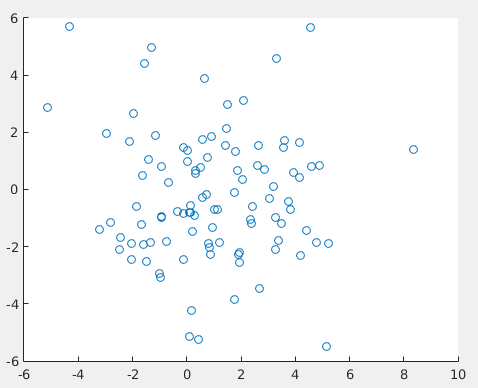
\includegraphics[scale=0.5]{Imgs/010301.png}
	\caption{Histogram for Samples from $N(\mu_1, \Sigma_1)$}
	\label{fig:4}
\end{figure}

Also, figure \ref{fig:5}, represents the histogram of generated samples from Gaussian distribution with $\mu_2$ and $\Sigma_2$. 
\begin{figure}[H]
	\centering
	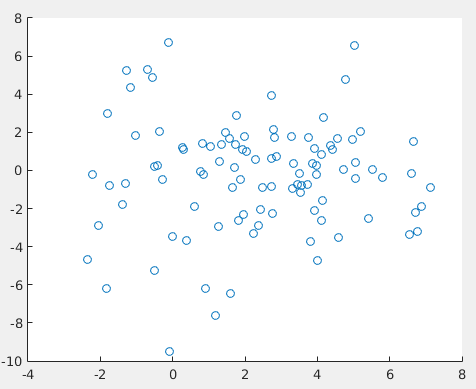
\includegraphics[scale=0.5]{Imgs/010302.png}
	\caption{Histogram for Samples from $N(\mu_2, \Sigma_2)$}
	\label{fig:5}
\end{figure}
}
\newpage
\problemAnswer{
Finally, figure \ref{fig:6} illustrates density of generated data from Gaussian distribution with $\mu_3$ and $\Sigma_3$.
\begin{figure}[H]
	\centering
	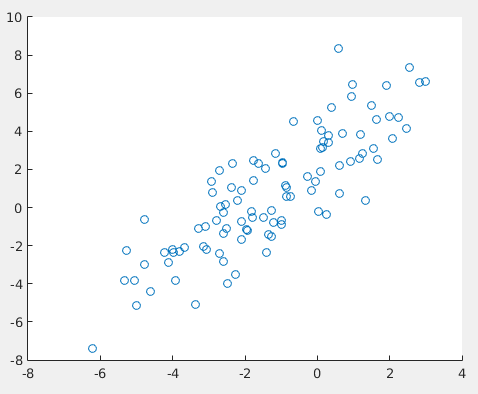
\includegraphics[scale=0.5]{Imgs/010303.png}
	\caption{Histogram for Samples from $N(\mu_3, \Sigma_3)$}
	\label{fig:6}
\end{figure}

}

\end{homeworkProblem}


\begin{homeworkProblem}

Compute the sample mean and sample covariance matrix of problem 3. (Using MATLAB).


\vspace{10pt}
\Large{Solution}
\vspace{10pt}

\problemAnswer{
The sample mean ($\hat{\mu_1}$) and sample covariance ($\hat{\Sigma_1}$) of the first case in the problem 3 has been calculated using \textit{mean} and \textit{cov} functions in MATLAB respectively as in \eqref{eq:1}
\\
\begin{align*}
&\hat{\mu_1} = \left[ \begin{matrix}
1.1857 \\
0.0655
\end{matrix} \right] \\
&\hat{\Sigma_1} = \left[ \begin{matrix}
4.1571 & 0.5437 \\
0.5437 & 5.0397
\end{matrix} \right]
\numberthis
\label{eq:1}
\end{align*}

The sample mean ($\hat{\mu_2}$) and sample covariance ($\hat{\Sigma_2}$) of the second case in the problem 3 has been calculated using \textit{mean} and \textit{cov} functions in MATLAB respectively as in \eqref{eq:2}

}
\problemAnswer{
\begin{align*}
&\hat{\mu_2} = \left[ \begin{matrix}
2.1662 \\
0.3162
\end{matrix} \right] \\
&\hat{\Sigma_2} = \left[ \begin{matrix}
5.0991 & 0.4390 \\
0.4390 & 9.3366
\end{matrix} \right]
\numberthis
\label{eq:2}
\end{align*}
The sample mean ($\hat{\mu_3}$) and sample covariance ($\hat{\Sigma_3}$) of the third case in the problem 3 has been calculated using \textit{mean} and \textit{cov} functions in MATLAB respectively as in \eqref{eq:3}
\\
\begin{align*}
&\hat{\mu_3} = \left[ \begin{matrix}
-1.2534 \\
0.8770
\end{matrix} \right] \\
&\hat{\Sigma_3} = \left[ \begin{matrix}
5.0800 & 6.1385 \\
6.1385 & 10.7987
\end{matrix} \right]
\numberthis
\label{eq:3}
\end{align*}

}

\end{homeworkProblem}



\begin{homeworkProblem}
Use the normal distribution to approximate the binomial distribution and find the probability of getting 12 to 15 heads out of 20 flips. Compare this to what you get when you calculate the probability using the binomial distribution

\vspace{10pt}
\Large{Solution}
\vspace{10pt}

\problemAnswer{
Let $Y$ the random variable indicating head counts in 20 flips of a fair coin. Therefore, $Y \propto B(20,0.5)$. The figure \ref{fig:7} displays its distribution schema. This distribution can be approximated with a normal distribution with $\mu = 10$ and $\sigma = \sqrt{5}$ which is shown with a line in figure \ref{fig:7}

\begin{figure}[H]
	\centering
	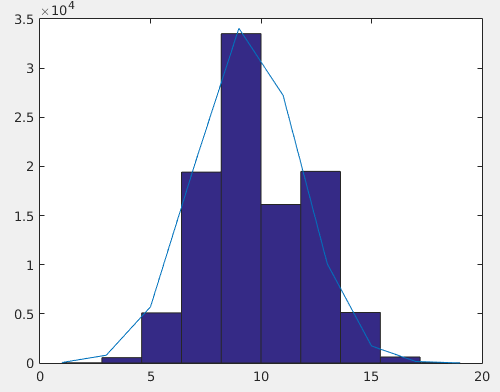
\includegraphics[scale=0.5]{Imgs/010501.png}
	\caption{Histogram of Distribution $B(20, 0.5)$. The line indicates a normal distribution $N(10, 5)$}
	\label{fig:7}
\end{figure}

According to this illustration, $Pr(12 \leq Y \leq 15)$ in binomiad distribution can be approximated using $Pr(11.5 \leq Y \leq 15.5)$ in normal distribution. which is :
\begin{align*}
Pr(11.5 \leq Y \leq 15.5) &= Pr(Y < 15.5) - Pr(Y \leq 11.5) \\
&= 0.9930 - 0.7488 = 0.2442 
\end{align*}

When accomplishing these calculations in binomial distribution directly we have:
\begin{align*}
Pr(12 \leq Y \leq 15) &= Pr(Y \leq 15) - Pr(Y \leq 11) \\
&= 0.9941 - 0.7483 = 0.2458 
\end{align*}

As its clear, the results are quite close to each other.


}
\end{homeworkProblem}


\begin{homeworkProblem}
\begin{itemize}
\item 
Compute eigenvalues and eigenvectors of $A = \left[ \begin{smallmatrix} 
2 & 0 & 0 \\
-1 & 3 & 3 \\
6 & -6 & -6 \end{smallmatrix} \right]$ and compare your results with Matlab outputs.

\item
a $2 * 2$ matrix A matrix has $\lambda_1 = 2$ and $\lambda_2 = 5$, with corresponding eigenvectors $v_1 = \left[ \begin{smallmatrix} 1 & 0 \end{smallmatrix} \right]^T $ and $v_2 = \left[ \begin{smallmatrix} 1 & 1 \end{smallmatrix} \right]^T$ . Find A.
\end{itemize}
\vspace{10pt}
\Large{Solution}
\vspace{10pt}

\problemAnswer{
To calculate eigenvalues:
\begin{align*}
|A - \lambda I|  &= 0  \rightarrow \\
&|\left[
\begin{matrix}
2 & 0 & 0 \\
-1 & 3 & 3 \\
6 & -6 & -6 
\end{matrix}
\right]
-
\left[
\begin{matrix}
\lambda & 0 & 0 \\
0 & \lambda & 0 \\
0 & 0 & \lambda 
\end{matrix}
\right]|
= 0 \rightarrow\\
&(2-\lambda)\cdot((3-\lambda)(-6-\lambda)-18) = 0 \rightarrow\\
&(2-\lambda)\cdot(3\lambda + \lambda^2) = 0 \rightarrow \\
&\lambda_1 = 2 \\
&\lambda_2 = 0 \\
&\lambda_3 = -3
\end{align*}
To calculate eigenvectors :
\begin{align*}
A v &= \lambda v  \rightarrow (A - \lambda_1 I) v_1 = 0 \rightarrow \\
&\left[
\begin{matrix}
2 - \lambda_1 & 0 & 0 \\
-1 & 3 - \lambda_1 & 3 \\
6 & -6 & -6 - \lambda_1 
\end{matrix}
\right]
\left[
\begin{matrix}
v_{11} \\
v_{12} \\
v_{13}
\end{matrix}
\right]
=
0 \rightarrow \\
&\left[
\begin{matrix}
 0 & 0 & 0\\
-1 & 1 & 3 \\
6 & -6 & -8 
\end{matrix}
\right]
\left[
\begin{matrix}
v_{11} \\
v_{12} \\
v_{13}
\end{matrix}
\right]
= 0 \rightarrow \\
&v_{11} = v_{12} , v_{13} = 0
\\
\end{align*}
}
\newpage
\problemAnswer{
Which is consistent with MATLAB output:
\begin{center}
$
v_1 = \left[ 
\begin{matrix}
0.7071 \\
0.7071 \\
0
\end{matrix}
\right]
$
\end{center}
For other eigenvectors:
\begin{align*}
A v &= \lambda v  \rightarrow (A - \lambda_2 I) v_2 = 0 \rightarrow \\
&\left[
\begin{matrix}
2 - \lambda_2 & 0 & 0 \\
-1 & 3 - \lambda_2 & 3 \\
6 & -6 & -6 - \lambda_2 
\end{matrix}
\right]
\left[
\begin{matrix}
v_{21} \\
v_{22} \\
v_{23}
\end{matrix}
\right]
=
0 \rightarrow \\
&\left[
\begin{matrix}
 2 & 0 & 0\\
-1 & 3 & 3 \\
6 & -6 & -6 
\end{matrix}
\right]
\left[
\begin{matrix}
v_{21} \\
v_{22} \\
v_{23}
\end{matrix}
\right]
= 0 \rightarrow \\
&v_{22} = -v_{23} , v_{21} = 0
\\
\end{align*}
Which is consistent with MATLAB output:
\begin{center}
$
v_2 = \left[ 
\begin{matrix}
0 \\
-0.7071 \\
0.7071
\end{matrix}
\right]
$
\end{center}
For the third eigenvectors:
\begin{align*}
A v &= \lambda v  \rightarrow (A - \lambda_3 I) v_3 = 0\rightarrow \\
&\left[
\begin{matrix}
2 - \lambda_3 & 0 & 0 \\
-1 & 3 - \lambda_3 & 3 \\
6 & -6 & -6 - \lambda_3 
\end{matrix}
\right]
\left[
\begin{matrix}
v_{31} \\
v_{32} \\
v_{33}
\end{matrix}
\right]
=
0 \rightarrow \\
&\left[
\begin{matrix}
 5 & 0 & 0\\
-1 & 6 & 3 \\
6 & -6 & -3 
\end{matrix}
\right]
\left[
\begin{matrix}
v_{31} \\
v_{32} \\
v_{33}
\end{matrix}
\right]
= 0 \rightarrow \\
& v_{31} = 0 \\
\end{align*}
}
\newpage
\problemAnswer{
Which is consistent with MATLAB output:
\begin{center}
$
v_3 = \left[ 
\begin{matrix}
0 \\
0.4472 \\
-0.8944
\end{matrix}
\right]
$
\end{center}

\begin{small}
(The MATLAB code has been attached to the submitted zip file.)
\end{small}

To calculate matrix A:
\begin{align*}
&\left[
\begin{matrix}
a_{11} - \lambda_1 & a_{12} \\
a_{21} & a_{22} - \lambda_1 \\
\end{matrix}
\right]
\left[
\begin{matrix}
v_{11} \\
v_{12}
\end{matrix}
\right]
=
0 \rightarrow \\
&\left[
\begin{matrix}
a_{11} - 2 \\
a_{21}
\end{matrix}
\right]
=
0 \rightarrow \\
&a_{21} = 0 , a_{11} = 2 \\
&\left[
\begin{matrix}
2 - \lambda_2 & a_{12} \\
0 & a_{22} - \lambda_2 \\
\end{matrix}
\right]
\left[
\begin{matrix}
v_{21} \\
v_{22}
\end{matrix}
\right]
=
0 \rightarrow \\
&\left[
\begin{matrix}
a_{12} - 3 \\
a_{22} - 5
\end{matrix}
\right]
=
0 \rightarrow \\
&a_{12} = 3 , a_{22} = 5 \\
&A = \left[
\begin{matrix}
2 & 3 \\
0 & 5
\end{matrix}
\right]
\end{align*}
}
\end{homeworkProblem}

\begin{homeworkProblem}
Let $ f(x,y) = \twopartdef{c(x+y)}{0 < x < 1; 0 < y < 1 }{0}{otherwise} $
Find appropriate constant $c$, marginal density $f_X(x)$, conditional density $f_{X|Y}(y)$. Are $X$ and $Y$ independent? What is the probability $Pr(X < 0.5 | Y = 0.5)$?
\\
\vspace{10pt}
\Large{Solution}
\vspace{10pt}

\problemAnswer{
The constant c: 
\begin{align*}
&\int_{-\infty}^{+\infty} \int_{-\infty}^{+\infty} f(x, y) dx dy = 1 \rightarrow \int_0^1 \int_0^1 c(x+y) dx dy = 1 \rightarrow \\
&\int_0^1 \frac{c}{2} + cy dy = 1 \rightarrow c = 1. 
\end{align*}
The marginal density $f_X(x)$: 
\begin{align*}
f_X(x) &= \int_{-\infty}^{+\infty} f(x, y) dy = \int_0^1 (x+y) dy\rightarrow \\
&f_X(x) = x + 0.5 , 0 \leq x \leq 1\\
\end{align*}
The conditional density $f_{X|Y}(x|y)$: 
\begin{align*}
f_{X|Y}(x|y) &= \frac{f_{X,Y}(x, y)}{f_Y(y)}\\
&f_Y(y) = y + 0.5 \rightarrow \\
f_{X|Y}(x|y) &= \frac{x + y}{y + 0.5} , 0 \leq x \leq 1 , 0 \leq y \leq 1 and 0 otw\\
\end{align*}

}
\end{homeworkProblem}


\begin{homeworkProblem}
Gaussians: Recall the multivariate Gaussian for a vector $ x \in R^n$ .\\

\begin{itemize}
\item 
Let $y = v_i^T \cdot x$ , where $v_i$ is an eigenvector of $\Sigma$ with an eigenvalue of $\lambda_i$. Find the probability density of $p(y)$.

\item Let $x$ be a zero mean guassian random vector with a isotropic covariance $( \Sigma = I )$. Let
$y=Ax+b$. Compute the mean and variance of $y$.

\item (MATLAB) Generate 500 random samples from a 2 dimensional Gaussian with an isotropic $\Sigma$ using matlab command randn. Transform the data as above with 
$b = \left[ \begin{smallmatrix}
0.5 \\
1
\end{smallmatrix} \right]$
and
$A = \left[ \begin{smallmatrix}
-5 & 5 \\
1 & 1
\end{smallmatrix} \right]$. plot the original and transformed points.
\end{itemize}


\vspace{10pt}
\Large{Solution}
\vspace{10pt}

\problemAnswer{
}
\end{homeworkProblem}


\begin{homeworkProblem}
If $X$ and $Y$ are independent and identically distributed with mean $\lambda$ and variance $\sigma^2$ , find $E[(X - Y )^2 ]$.
\vspace{10pt}
\Large{Solution}
\vspace{10pt}

\problemAnswer{
}
\end{homeworkProblem}


\begin{homeworkProblem}

Diagonalize the following two matrices simultaneously:
\begin{center}

$
\Sigma_1 = \left[ \begin{smallmatrix}
1 & 0.5 \\
0.5 & 1
\end{smallmatrix} \right]
$
and 
$
\Sigma_2 = \left[ \begin{smallmatrix}
1 + \sqrt{\frac{3}{4}} & 0.5 \\
0.5 & 1 - \sqrt{\frac{3}{4}} 
\end{smallmatrix} \right]
$


\end{center}
\vspace{10pt}
\Large{Solution}
\vspace{10pt}

\problemAnswer{
}
\end{homeworkProblem}


\begin{homeworkProblem}
Let $p(X)$ be $N_x (M, \Sigma)$ with
\begin{center}
$
x = \left[ \begin{smallmatrix}
x_1 \\
x_2 
\end{smallmatrix} \right]
$
,
$
M = \left[ \begin{smallmatrix}
m_1 \\
m_2
\end{smallmatrix} \right]
$
and 
$
\Sigma_2 = \left[ \begin{smallmatrix}
\sigma_1^2 & \rho \sigma_1 \sigma_2 \\
 \rho \sigma_1 \sigma_2  & \sigma_2^2 
\end{smallmatrix} \right]
$

\end{center}
Show that:
\\
$
p(x_1) = N_{x_1} (m_1, \sigma_1^2)$ (a marginal density)\\
$p(x_1|x_2) = N_{x_1} (m_1 + \rho \sigma_1 \frac{(x_2-m_2)}{\sigma_2} , \sigma_1^2(1 - \rho^2))$ (a conditional density)

\vspace{10pt}
\Large{Solution}
\vspace{10pt}

\problemAnswer{
}
\end{homeworkProblem}


\end{document}
